\section{Background}

\begin{frame}
    \frametitle{Machine Learning and Dynamical Systems}

    \begin{columns}[T] % align columns
        \begin{column}{.33\textwidth}
            {
                \color{nusblue}
                Machine Learning via Dynamical Systems
                \rule{\linewidth}{4pt}
            }
            \begin{itemize}
                \item Dynamical formulation of deep learning
                \item Dynamical analysis of learning algorithms
                \item Numerical analysis and architecture design
            \end{itemize}
        \end{column}%
        \hfill%
        \begin{column}{.33\textwidth}
            {
                \color{nusgreen}
                Machine Learning for Dynamical Systems
                \rule{\linewidth}{4pt}
            }
            \begin{itemize}
                \item Time series forecasting
                \item Sequence classification
                \item Sequence to Sequence models
            \end{itemize}
        \end{column}%
        \hfill%
        \begin{column}{.33\textwidth}
            {
                \color{nusorange}
                Machine Learning of Dynamical Systems
                \rule{\linewidth}{4pt}
            }
            \begin{itemize}
                \item Learning dynamical models from trajectories
                \item Learning reduced order models
            \end{itemize}
        \end{column}%
    \end{columns}
\end{frame}



\begin{frame}
    \frametitle{Sequence Modelling Applications}

    \begin{center}
        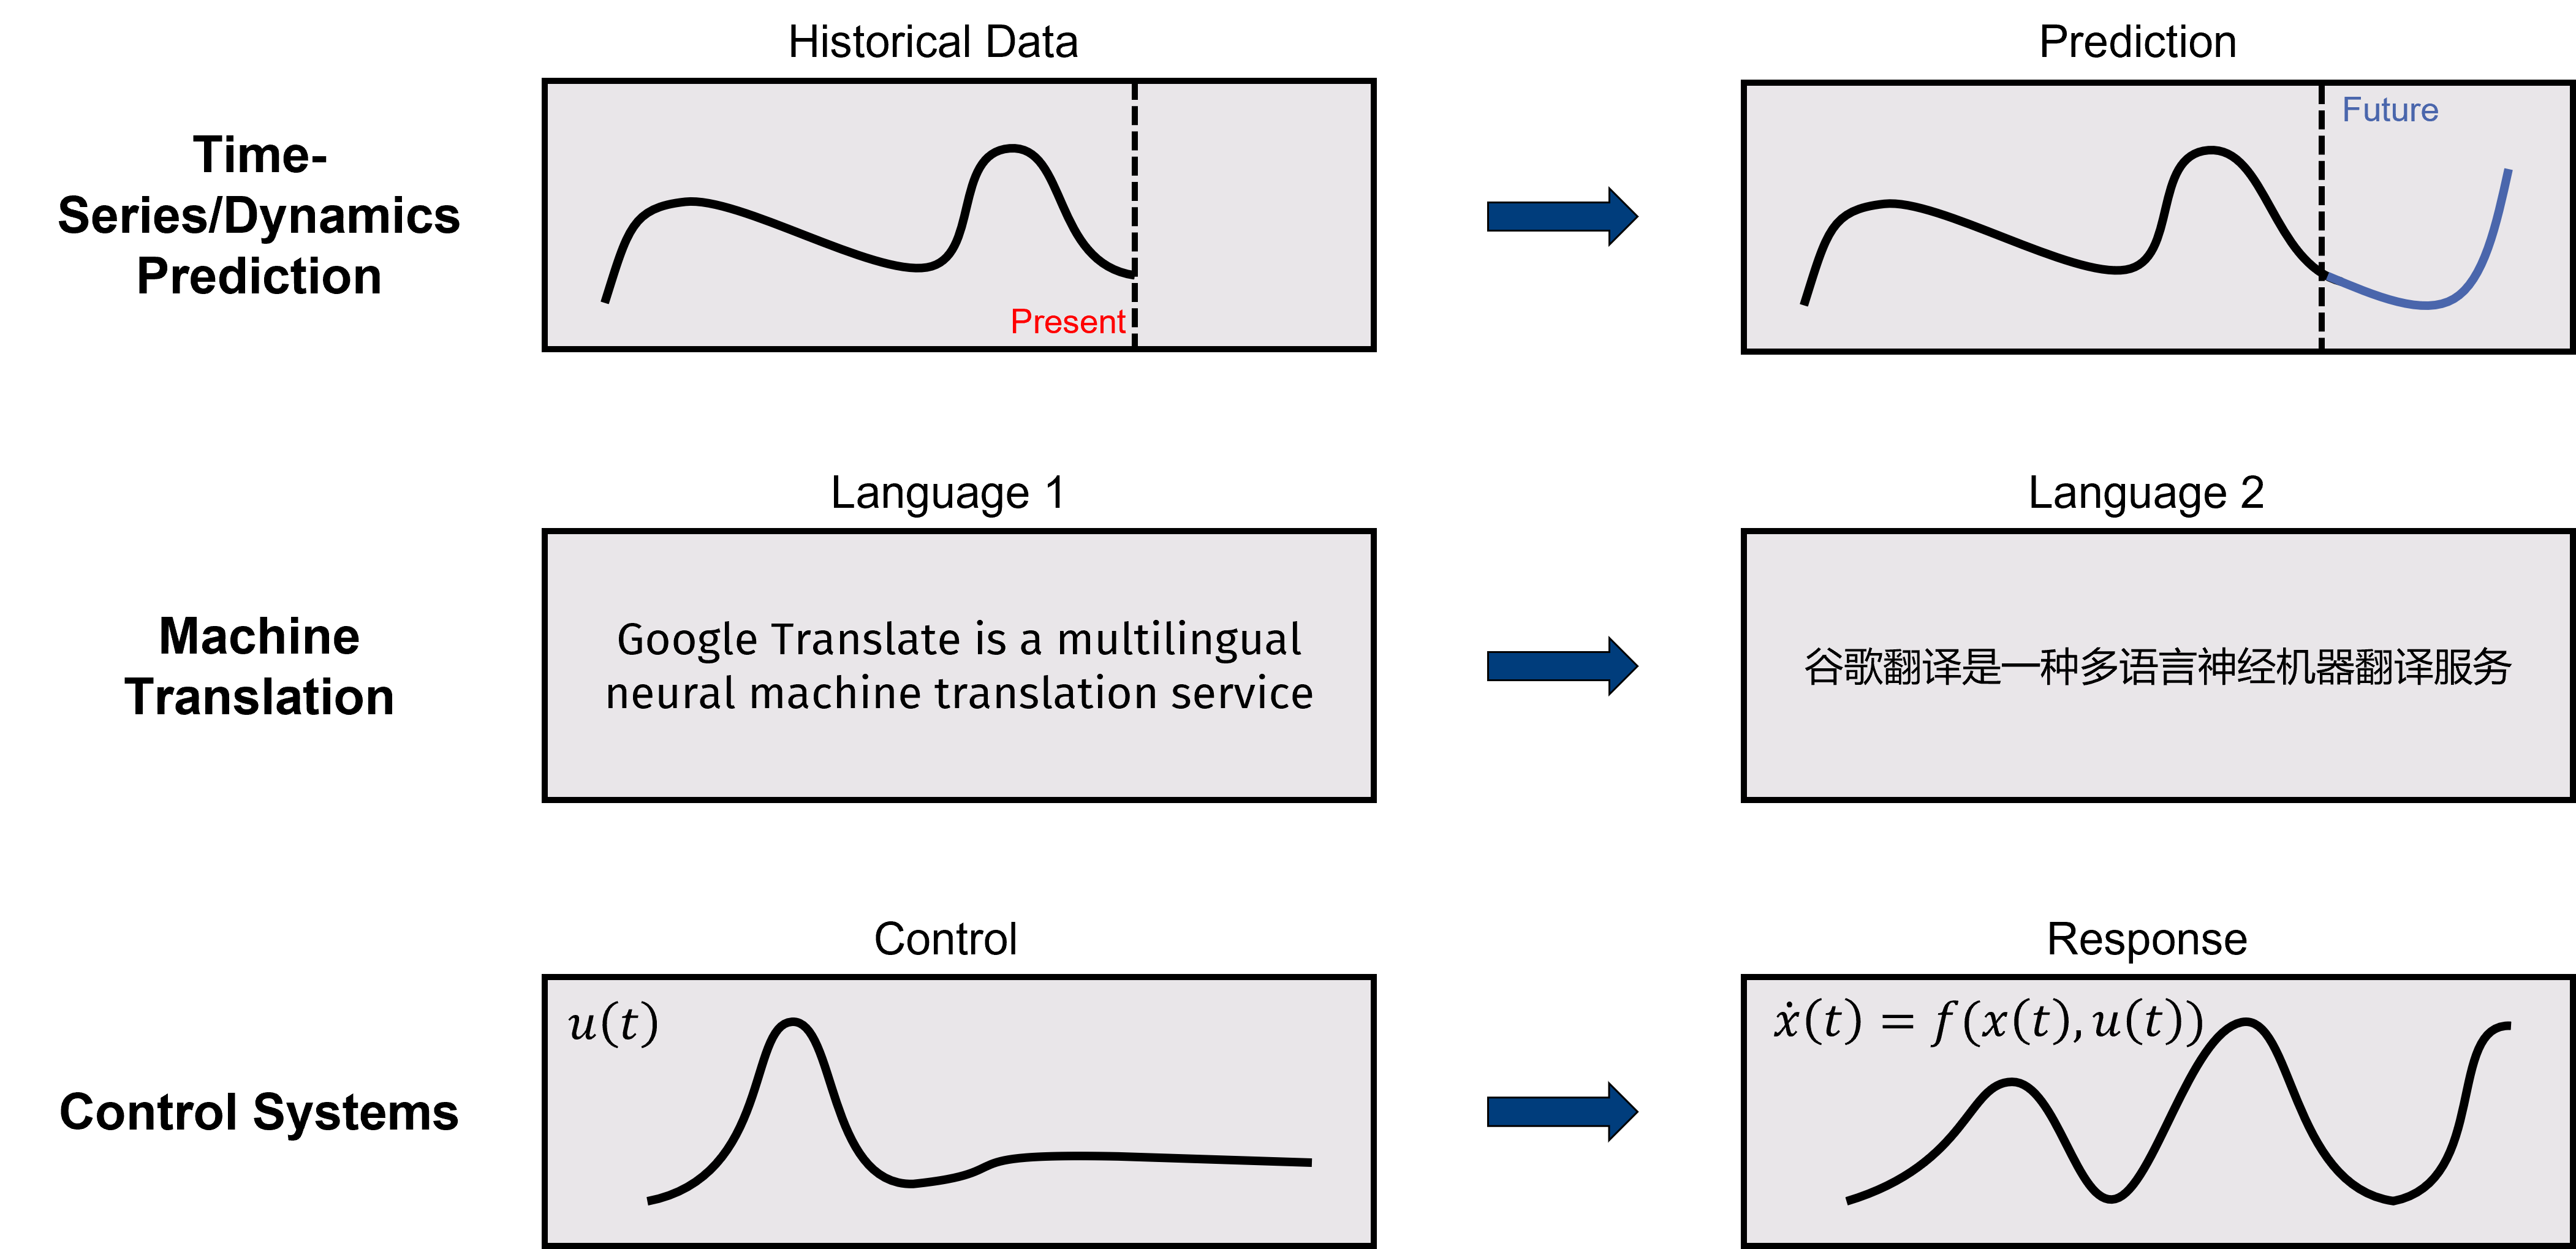
\includegraphics[width=\textwidth]{figures/seq_to_seq_applications.png}
    \end{center}

\end{frame}



\begin{frame}
    \frametitle{ML for DS: DL Architectures for Sequence Modelling}

    \begin{figure}
        \centering
        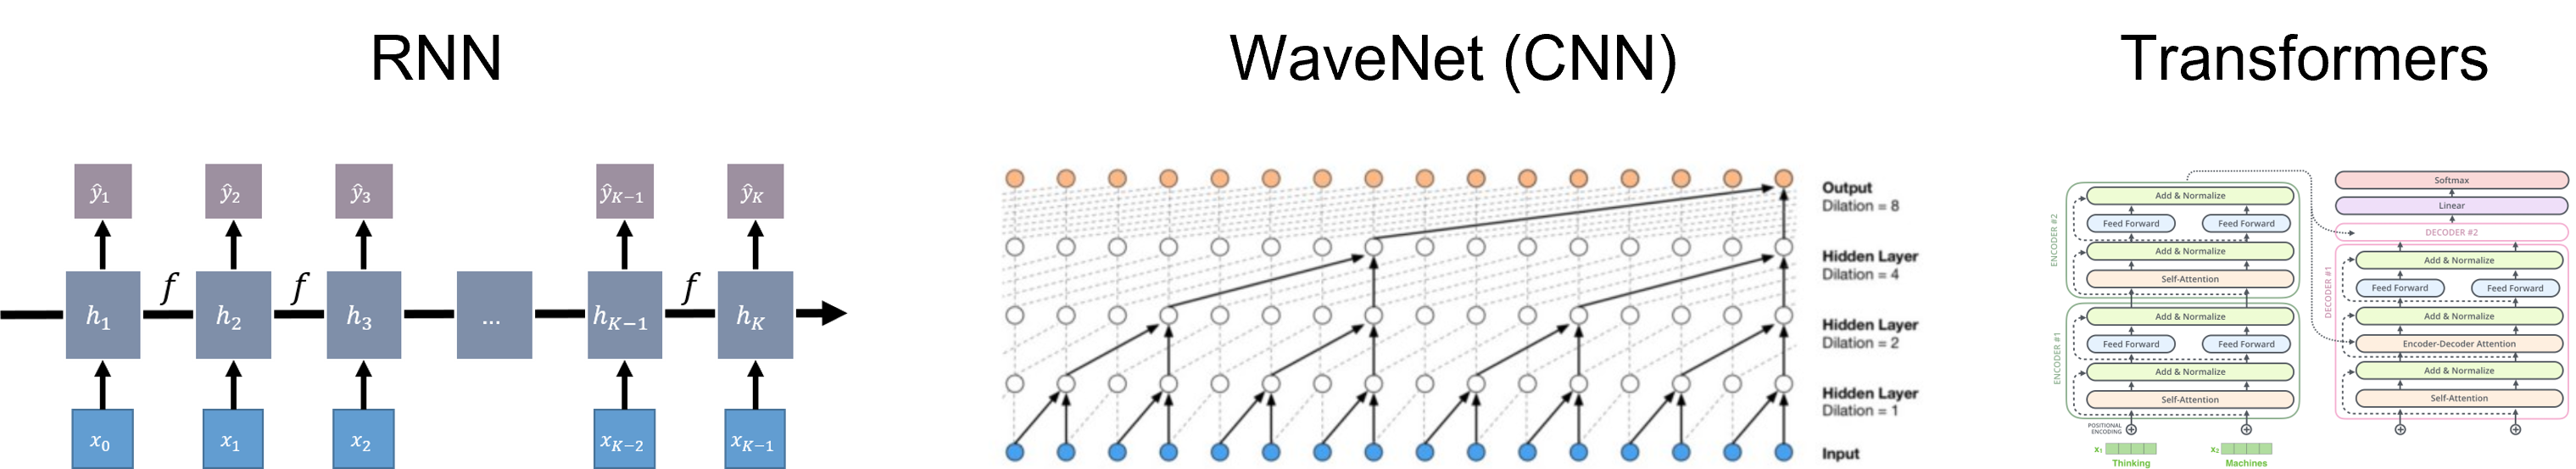
\includegraphics[width=\textwidth]{Figures/different_timeseries_archs.png}
    \end{figure}

    \begin{empheq}[box=\mymath]{gather*}
        \text{
            \textbf{General question:}
            How are they different? When should we use which?
        }
    \end{empheq}

\end{frame}

\begin{frame}
    \frametitle{Supervised Learning}

    \begin{center}
        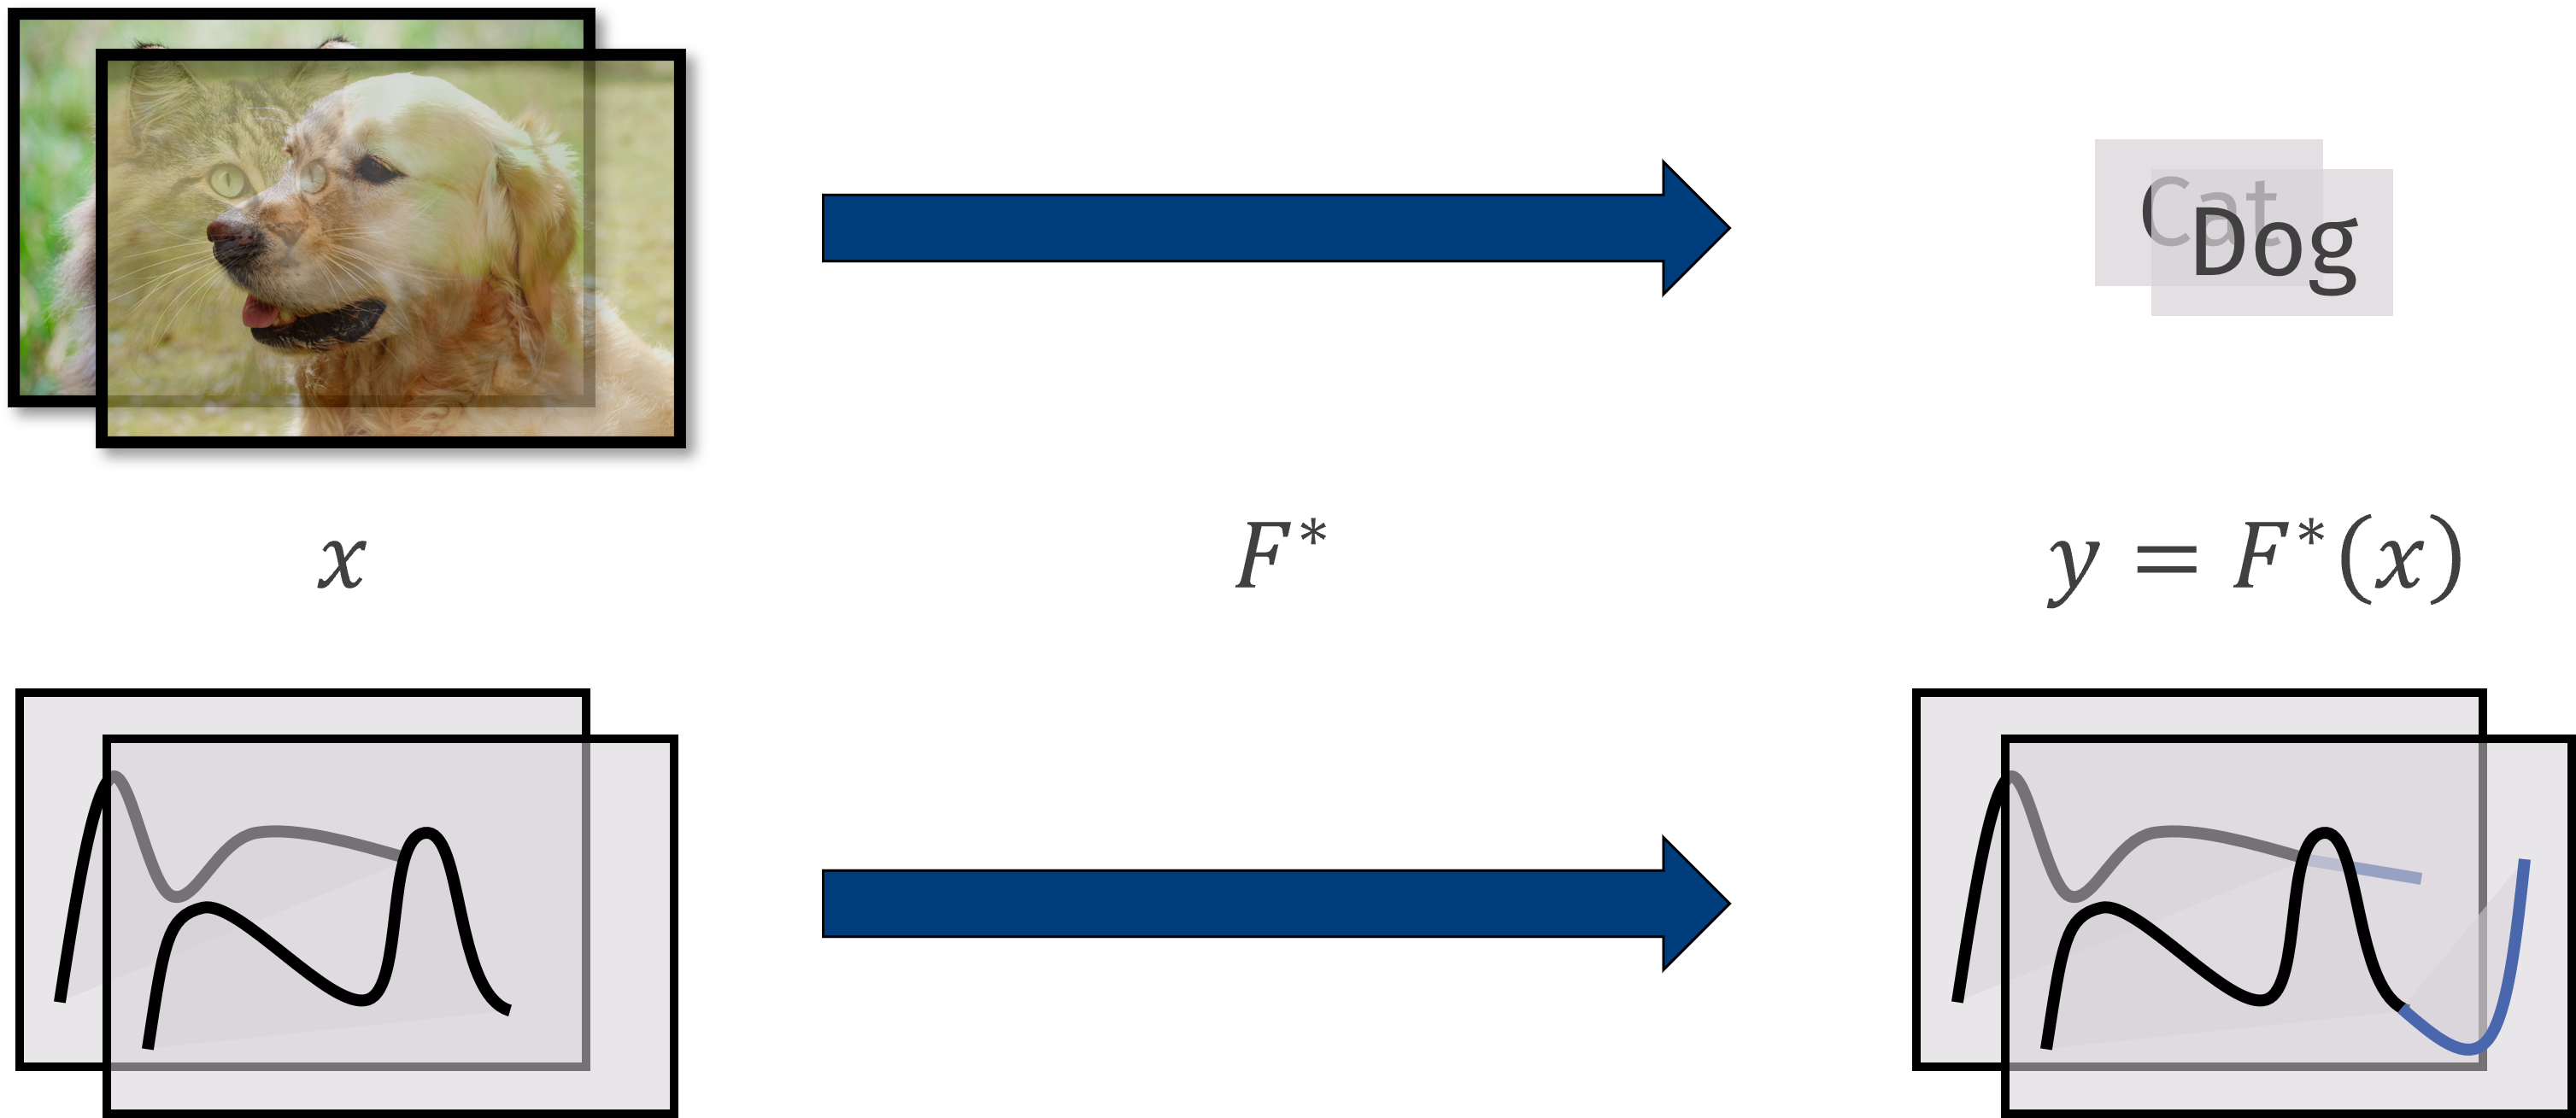
\includegraphics[width=0.8\textwidth]{Figures/target_function.png}
    \end{center}

    \pause{}

    \begin{empheq}[box=\mymath]{gather*}
        \text{
            \textbf{Goal:} Learn/approximate \alert{target} $F^*$
        }
    \end{empheq}


\end{frame}



\begin{frame}
    \frametitle{Modelling Static vs Dynamic Relationships}

    \begin{columns}[T] % align columns
        \begin{column}{.48\textwidth}
            {
                \color{nusorange}
                Static setting
                \rule{\linewidth}{4pt}
            }
            \begin{equation*}
                \begin{aligned}
                    &\text{\alert{(input)}}
                    \quad
                    &&x\in \Xcal = \R^d \\
                    &\text{\alert{(output)}}
                    \quad
                    &&y \in \Ycal = \R^n \\
                    &\text{\alert{(target)}}
                    \quad
                    &&y = F^*(x)
                \end{aligned}
            \end{equation*}
        \end{column}%
        \hfill%
        \pause{}
        \begin{column}{.48\textwidth}
            {
                \color{nusgreen}
                Dynamic setting
                \rule{\linewidth}{4pt}
            }
            \begin{equation*}
                \begin{aligned}
                    &\text{\alert{(input)}}
                    \quad
                    &&\*x = \{ x_k \in \R^d \} \in \Xcal
                    \\
                    &\text{\alert{(output)}}
                    \quad
                    &&\*y = \{ y_k \in \R^n \} \in \Ycal
                    \\
                    &\text{\alert{(target)}}
                    \quad
                    &&y_k = H_k^*(\*x) \quad \forall \quad k
                \end{aligned}
            \end{equation*}
        \end{column}%
    \end{columns}

    \vspace{.5cm}

    \pause{}

    Goal of supervised learning
    \begin{itemize}
        \item Static: learn/approximate $F^*$
        \item Dynamic: learn/approximate $\{ \Htar_k \}$
    \end{itemize}

\end{frame}


\begin{frame}
    \frametitle{Three Paradigms of Questions}

    \begin{overprint}
        \onslide<1>\centerline{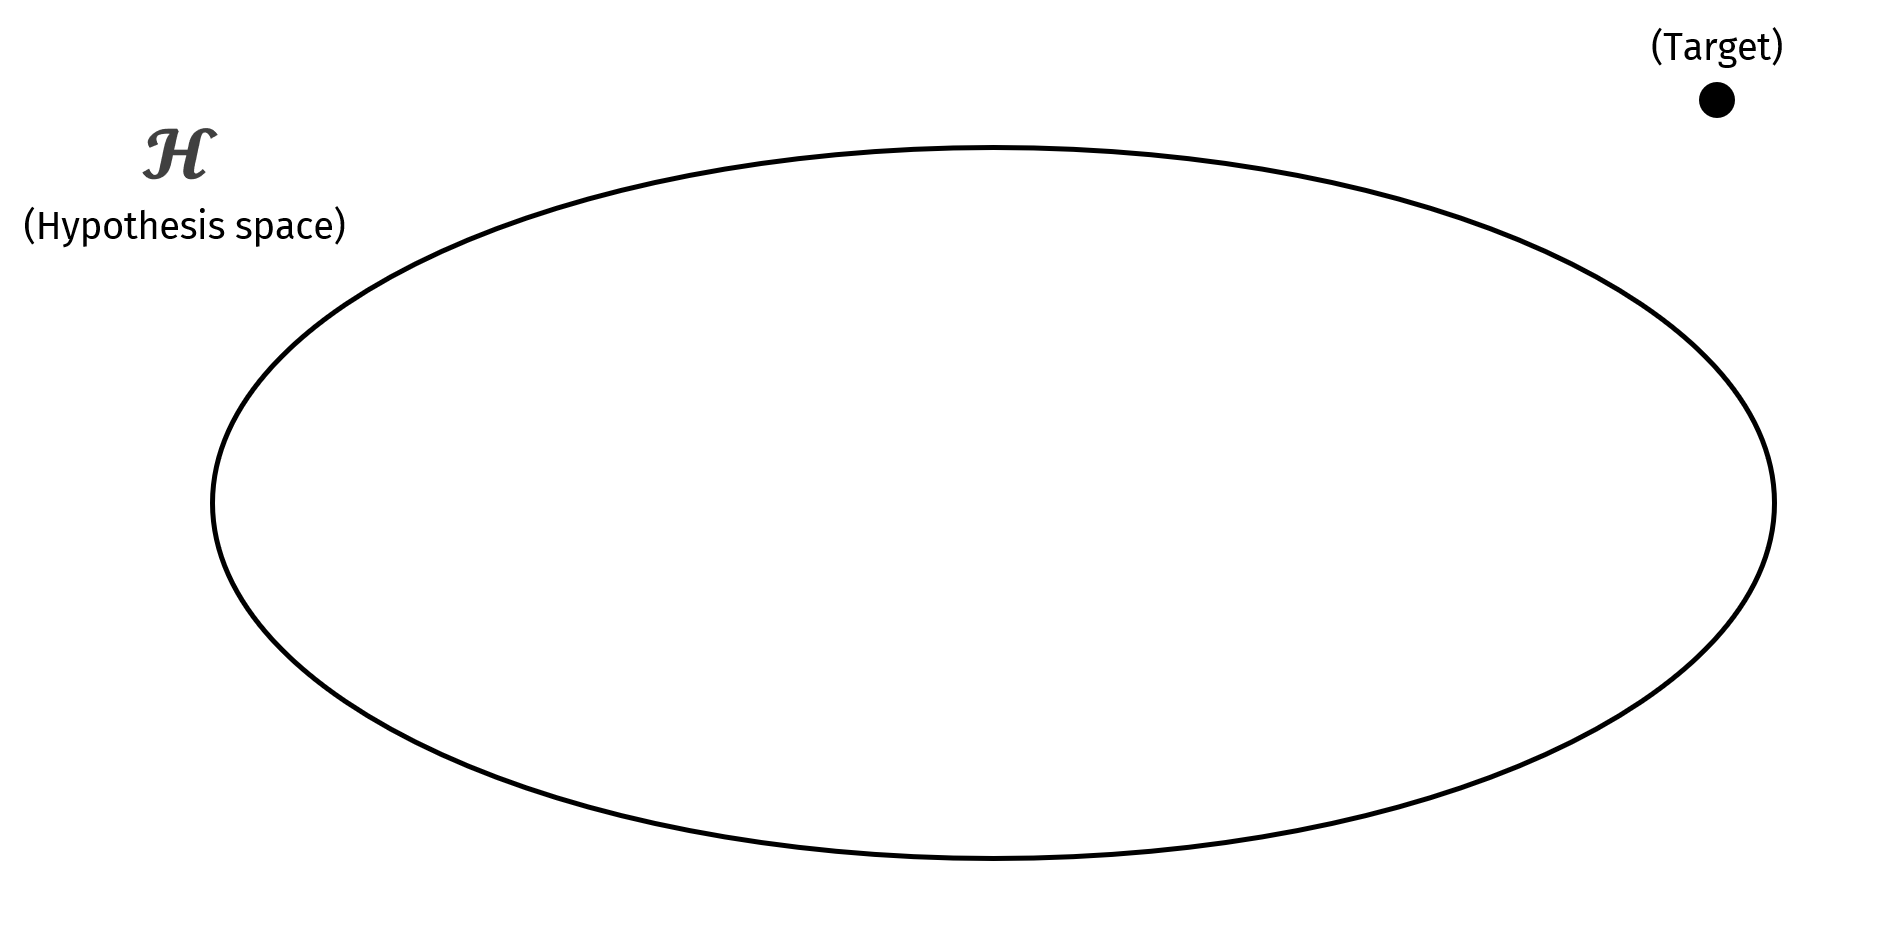
\includegraphics[width=\textwidth]{Figures/paradigm_1.png}}
        \onslide<2>\centerline{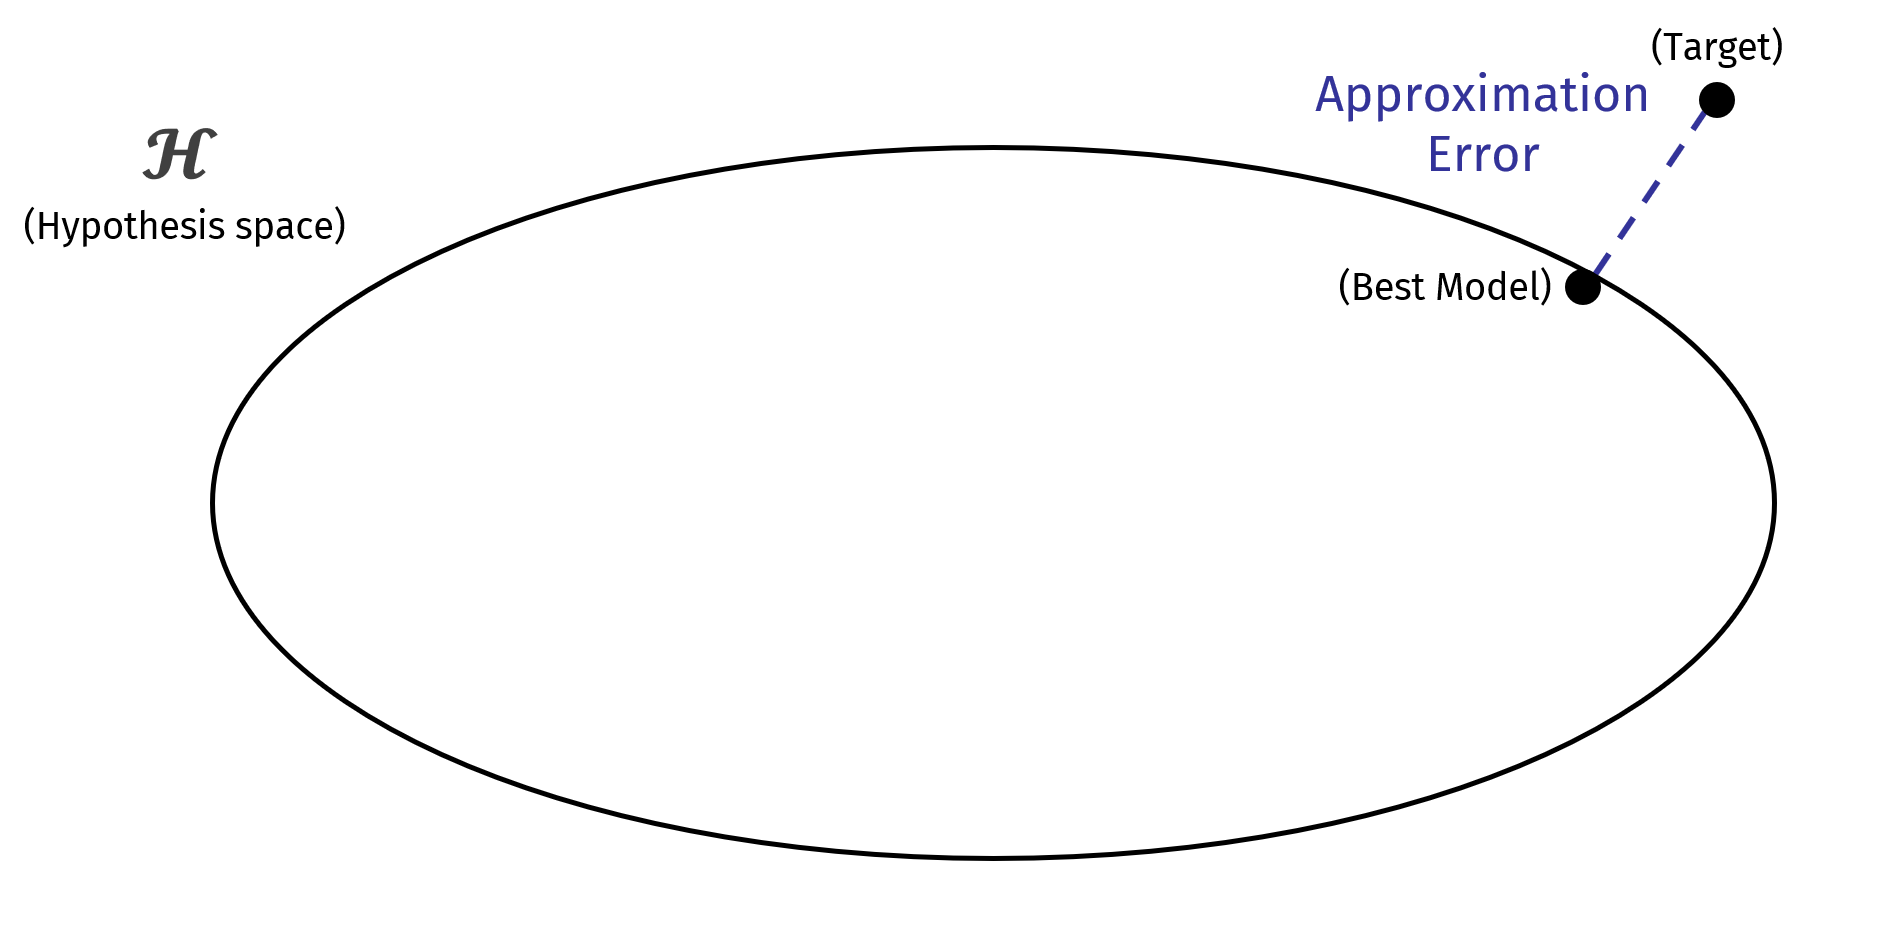
\includegraphics[width=\textwidth]{Figures/paradigm_2.png}}
        \onslide<3>\centerline{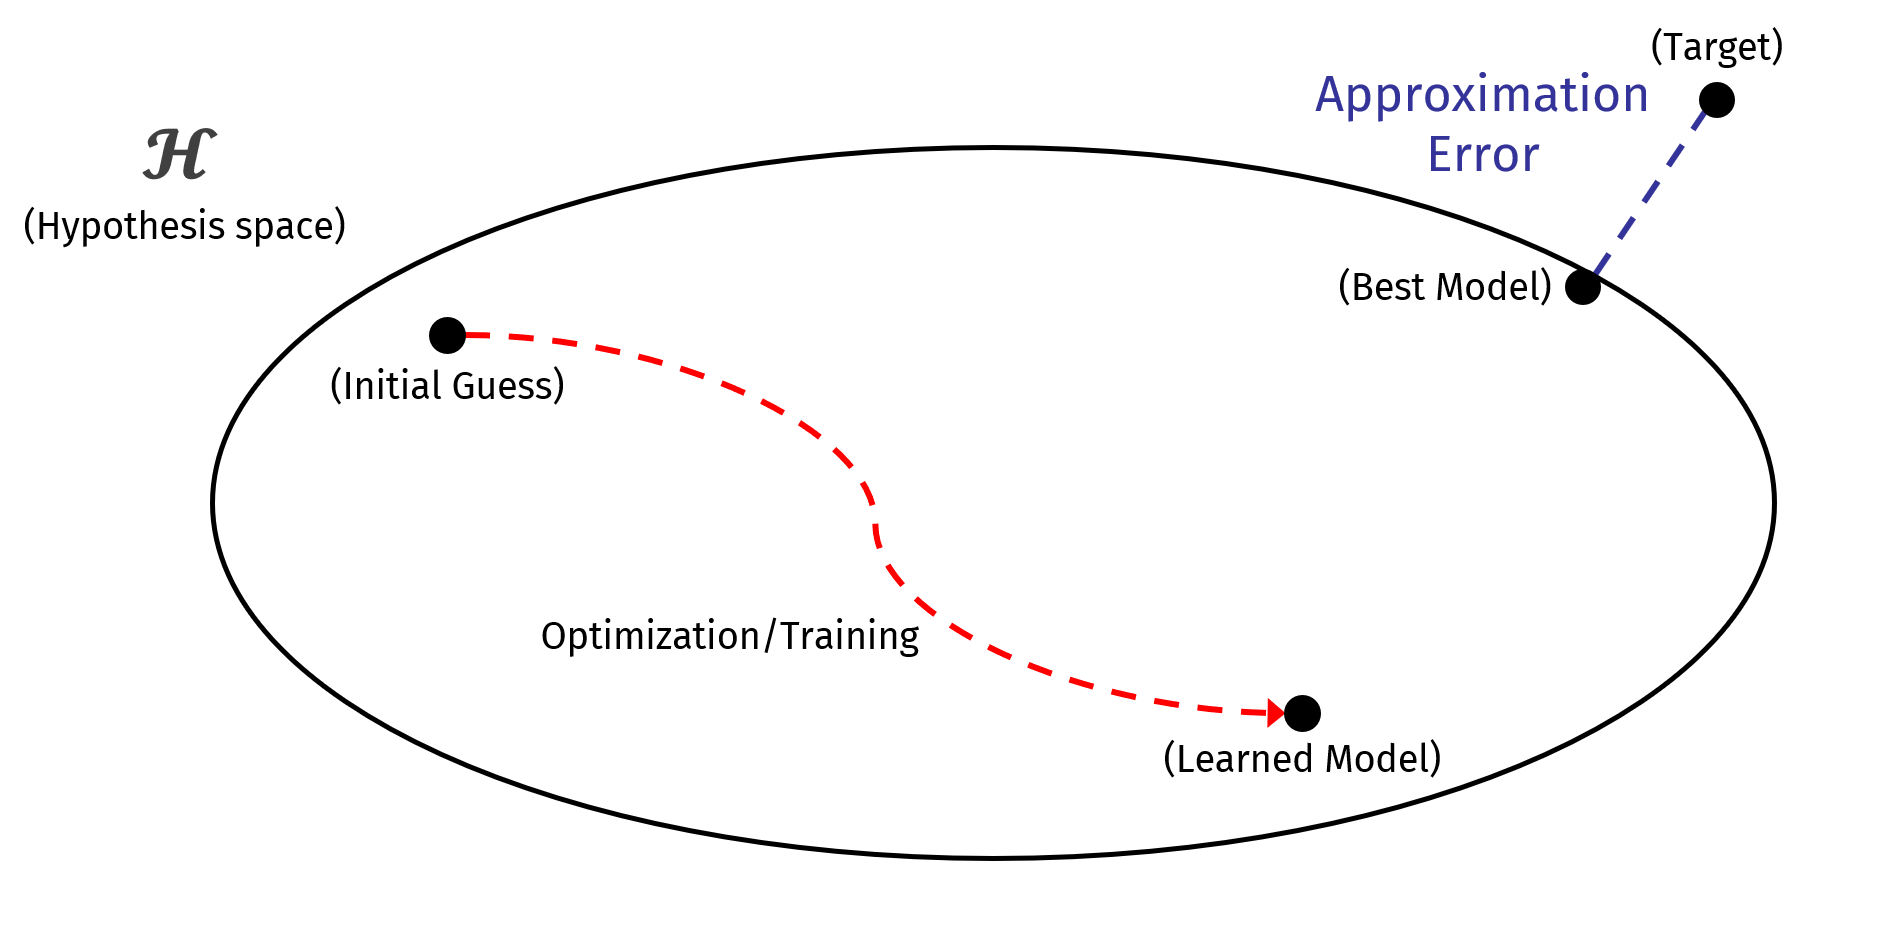
\includegraphics[width=\textwidth]{Figures/paradigm_3.png}}
        \onslide<4>\centerline{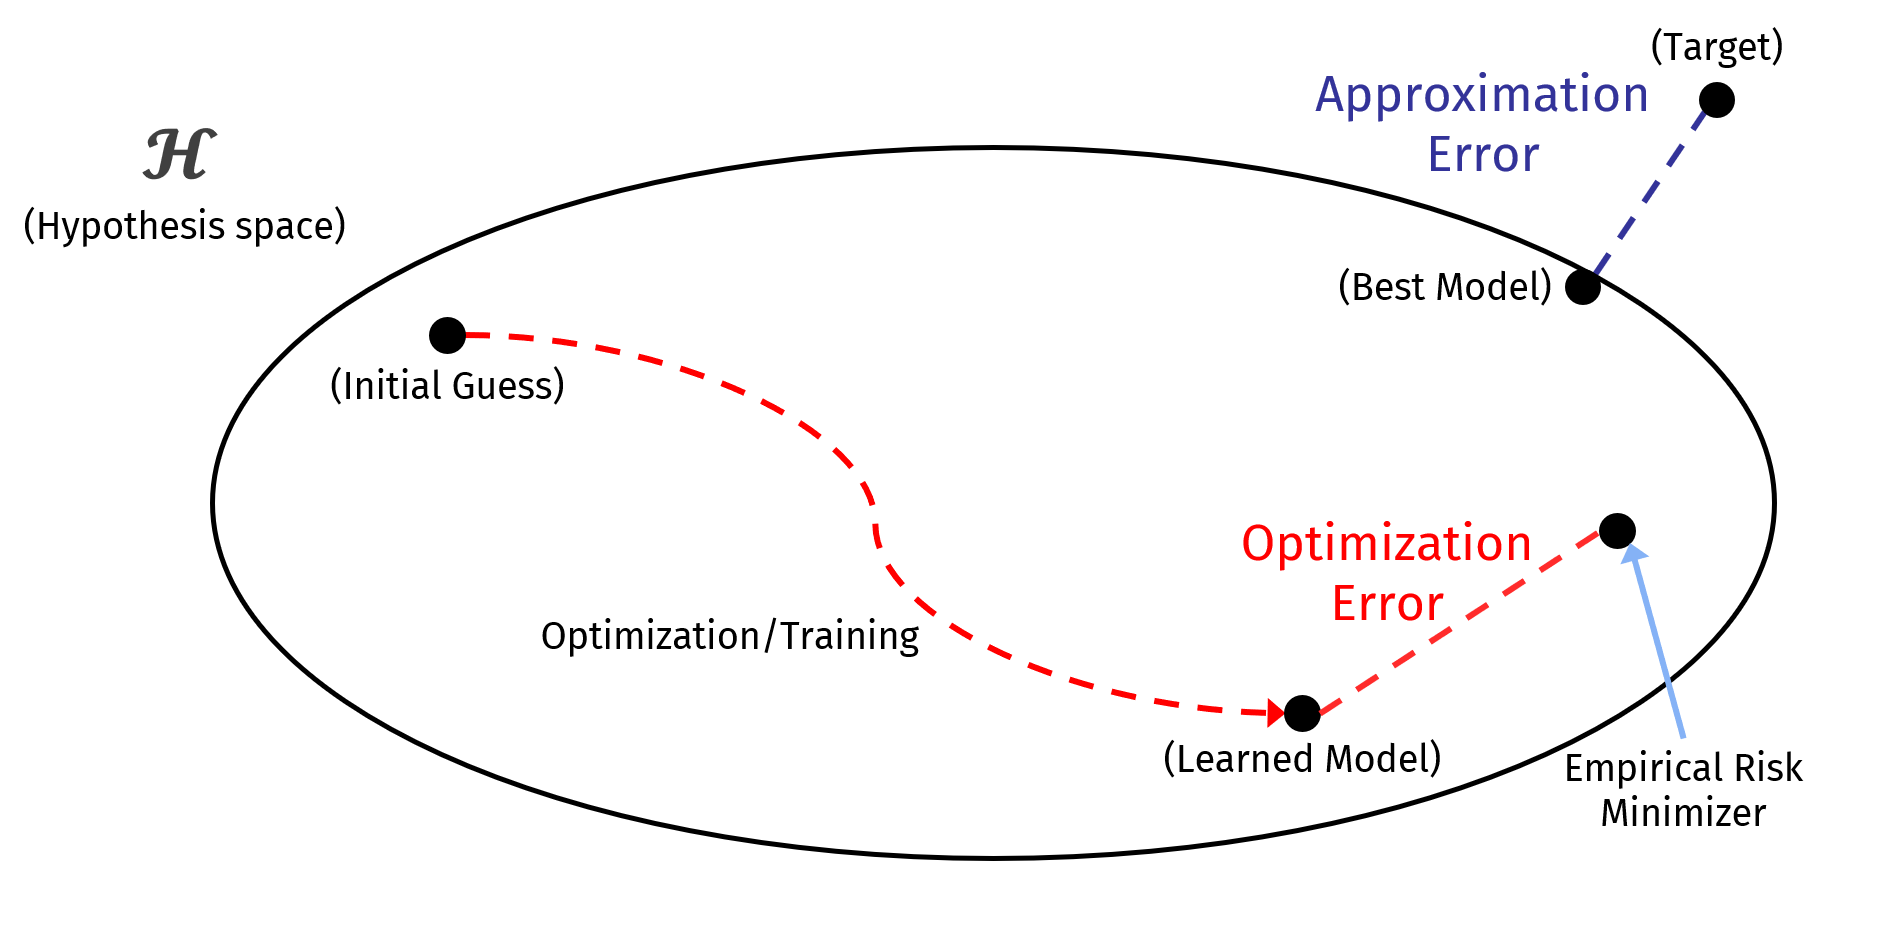
\includegraphics[width=\textwidth]{Figures/paradigm_4.png}}
        \onslide<5>\centerline{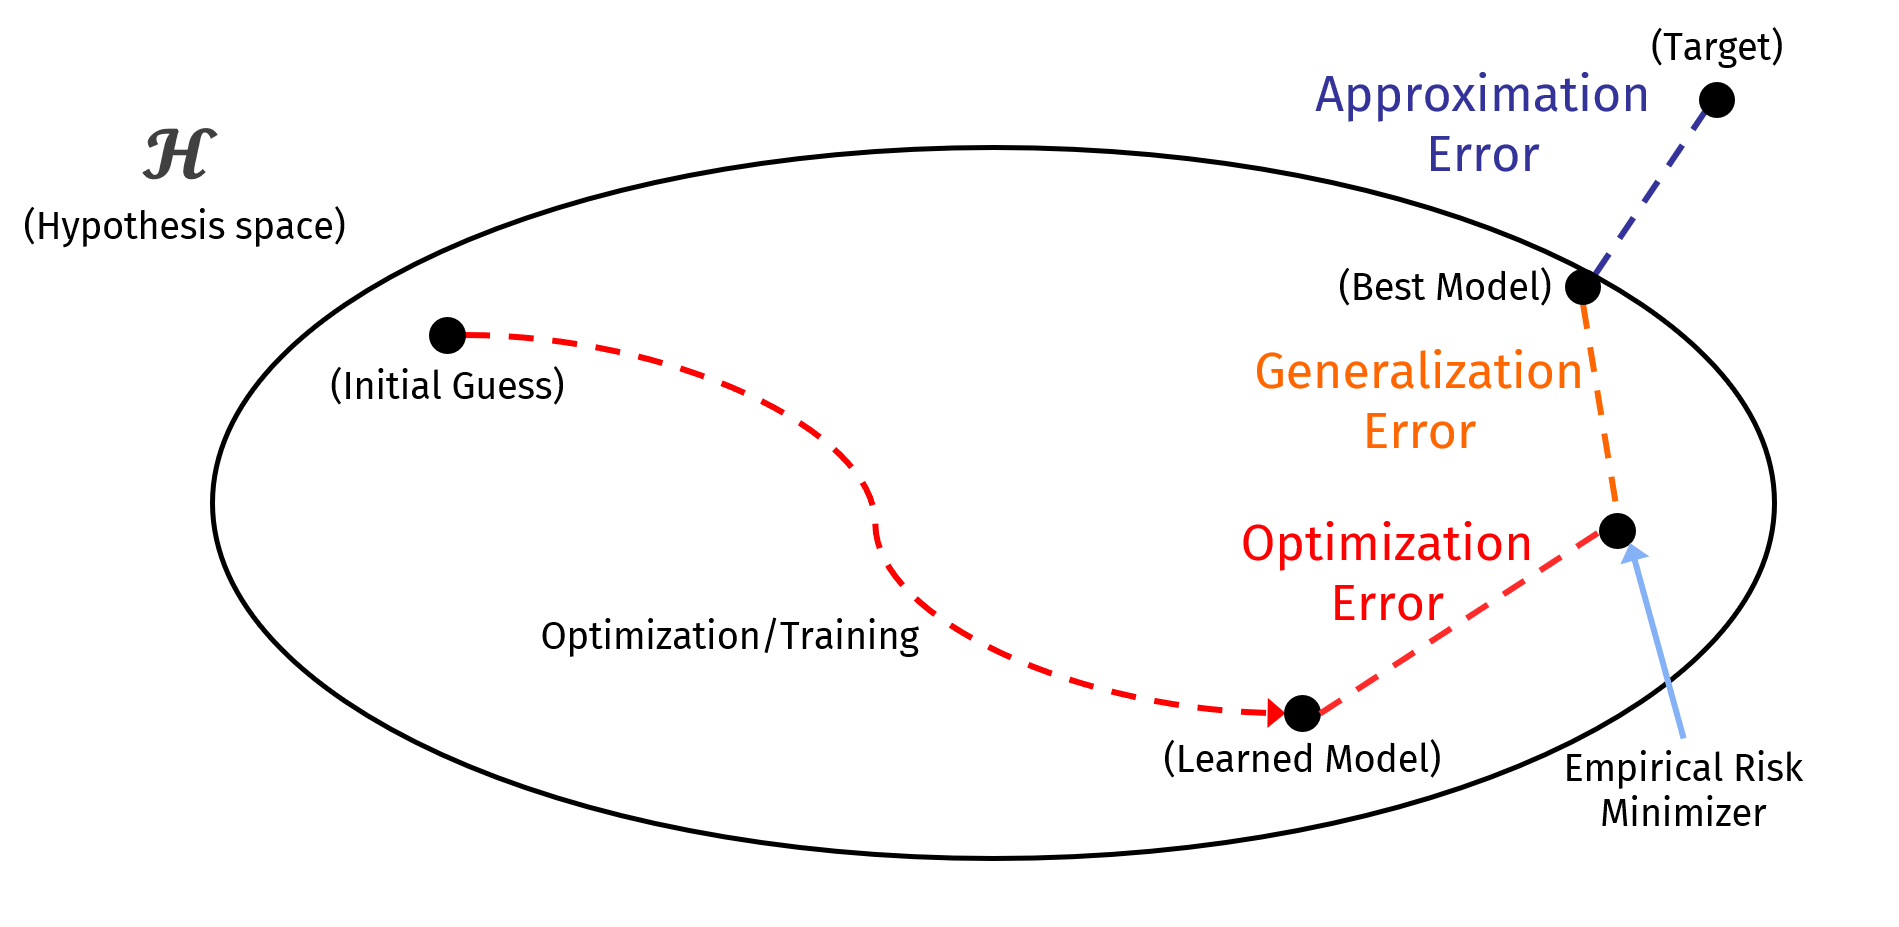
\includegraphics[width=\textwidth]{Figures/paradigm_5.png}}
    \end{overprint}
\end{frame}

\begin{frame}
    \frametitle{The Problem of Approximation}

    Given a hypothesis space $\Hcal$ and a target (concept) space $\Ccal$,
    we seek two types of approximation results
    \begin{itemize}
        \item Universal Approximation (Density)
        \begin{empheq}[box=\mymath]{gather*}
            \text{
                For each $H^* \in \Ccal$ and $\epsilon>0$, there exist $\wh{H} \in \Hcal$
                such that $\Vert H^* - \wh{H} \Vert \leq \epsilon$
            }
        \end{empheq}
        \pause{}
        \item Approximation Rates.
        Let ${\Hcal} = \cup_{m} {\Hcal}_{m}$,
        where ${\Hcal}_{m} \subset {\Hcal}_{m+1}$,
        $m$ measures size of hypothesis space (approximation budget)
        \begin{empheq}[box=\mymath]{gather*}
            \text{
                $
                    \inf_{\wh{H} \in {\Hcal}_m}
                    \Vert H^* - \wh{H}  \Vert
                    \leq
                    \text{Complexity}(H^*) \text{rate}(m)
                $,
                \qquad
                $\text{rate}(m) \rightarrow 0$
            }
        \end{empheq}
    \end{itemize}

\end{frame}

\begin{frame}
    \frametitle{Example: Approximation by Trigonometric Polynomials}

    Consider
    \begin{itemize}
        \item
        $\Ccal = C^{\alpha}_{\text{per}}([0,2\pi], \R)$ (periodic $C^{\alpha}$ functions)
        \item
        $
            {\Hcal}_m
            =
            \left\{
                \sum_{i=0}^{m-1} a_i \cos(i x) + b_i \sin(i x)
                :
                a_i,b_i \in \R
            \right\}
        $
        (trigonometric polynomials)
    \end{itemize}
    \pause{}
    Then, for each $H^* \in \Ccal$ \refhl{[Jackson, 1930]}
    \begin{equation*}
        \inf_{\wh{H} \in \Hcal_m}
        \| H^* - \wh{H} \|_{C}
        \leq
        \frac{C(\alpha)\max_{i\leq \alpha}\| {H}^{*(i)}\|_C}{m^\alpha}
    \end{equation*}
    Here, $\text{Complexity}(H^*) = \max_{i\leq\alpha} \| H^{*(i)} \|_C$
    and
    $\text{rate}(m) = m^{-\alpha}$.

    \pause{}
    \begin{empheq}[box=\mymath]{gather*}
        \text{
            \textbf{Insight:}
            Efficient approximation if $H^*$ is smooth (small gradient norm)
        }
    \end{empheq}
\end{frame}

\begin{frame}
    \frametitle{An Approximation Theory for Sequence Modelling}

    Our goal is to derive similar statements like Jackson's Theorem, but for
    \begin{itemize}
        \item $\Ccal$ $\rightarrow$ suitable classes of sequence relationships (functionals)
        \item $\Hcal$ $\rightarrow$ RNNs, CNNs/WaveNets, Encoder-Decoders, Transformers
    \end{itemize}

    \pause{}

    For each case, we aim to characterize
    \begin{itemize}
        \item What $\Ccal$ can be approximated (efficiently)?
        \item How does the complexity measure and rate estimate depend on different ${\Hcal}$?
        \item How to choose which $\Hcal$ to use in practice?
    \end{itemize}


\end{frame}
